% =============================================================================
%  CSE 200 -- BEAMER : COMPLETE ANNOTATED DEMO
% =============================================================================
%
%  The companion to cse200-demo.tex. Beamer is a document CLASS, not a
%  package, which is why it cannot share a file with the article demo.
%
%  COMPILE
%      latexmk -pdf cse200-demo-beamer.tex
%  or  pdflatex cse200-demo-beamer   (twice, for the table of contents)
%
%  WHAT CHANGES vs. an article
%      - the page becomes a "frame"
%      - content can appear in STAGES: one frame can produce several PDF pages
%      - \section produces no page of its own; it only feeds the ToC and the
%        navigation bar
%  WHAT DOES NOT CHANGE
%      - lists, maths, tables, figures, tikz all work exactly as before
%
%  This file draws on prev_onlines/beamer_tikZ_resources_21/BeamerTutorial and
%  .../beamer_tikZ_resources_23. It needs no external images.
% =============================================================================


% =============================================================================
%  CLASS AND THEME
% =============================================================================
%  aspectratio=169 gives a widescreen 16:9 deck (the default is 4:3).
%  Drop it for the classic shape:  \documentclass{beamer}
\documentclass[aspectratio=169,11pt]{beamer}

%  THEMES come in four independent layers:
%    \usetheme{...}       the overall look
%        Madrid Berkeley Berlin Copenhagen Frankfurt Singapore Warsaw
%        CambridgeUS metropolis default
%    \usecolortheme{...}  just the palette
%        seahorse lily dolphin beaver crane whale orchid rose
%    \usefonttheme{...}   just the fonts
%        professionalfonts serif structurebold
%    \useinnertheme{} / \useoutertheme{}
%        circles rectangles infolines miniframes split
%
%  NOTE: the metropolis theme (used in your own practice decks) needs XeLaTeX
%  or LuaLaTeX plus \usepackage{fontspec}; it will not build with pdflatex.
\usetheme{Madrid}
\usecolortheme{seahorse}

%  The little navigation arrows in the corner are almost never wanted.
%  An EMPTY template replaces them with nothing.
\setbeamertemplate{navigation symbols}{}

\usepackage{listings}
\usepackage{tikz}
\usetikzlibrary{positioning}

% -----------------------------------------------------------------------------
%  TITLE BLOCK
% -----------------------------------------------------------------------------
%  Most beamer title commands take an optional SHORT form in brackets: the
%  short form goes in the footline of every slide, the long form on the
%  title page.
\title[Beamer Demo]{We Love Beamer}
\subtitle{Every overlay, block and column construct, annotated}
\author[Zarif]{Zarif Ishmam}
\institute[CSE, BUET]{Department of Computer Science and Engineering, BUET}
\date{\today}

\begin{document}

% =============================================================================
%  TITLE AND OUTLINE
% =============================================================================
% \maketitle and \titlepage are interchangeable here.
\begin{frame}
    \maketitle
\end{frame}

% \tableofcontents is built from the \section commands between frames.
% It needs two compiles, exactly like an article's ToC.
\begin{frame}{Outline}
    \tableofcontents
\end{frame}


% =============================================================================
\section{Frames and overlays}
% =============================================================================

% TWO WAYS to title a frame -- they are identical:
%    \begin{frame}{Title}
%    \begin{frame} ... \frametitle{Title}
%
% \pause makes everything after it wait for the next click. This frame alone
% produces THREE PDF pages.
\begin{frame}{I am the TITLE}
    I am the FRAME. \pause I build up beamer presentations. \pause It is paused.
\end{frame}

\begin{frame}
    \frametitle{The other way to set a title}
    \framesubtitle{and a subtitle underneath it}
    Same result, different syntax.
\end{frame}

% -----------------------------------------------------------------------------
%  \setbeamercovered{transparent}
%  Without it, not-yet-revealed material is INVISIBLE (a blank gap).
%  With it, the material is DIMMED, so the audience can see what is coming.
%  It is a switch: everything after it in the document is affected.
% -----------------------------------------------------------------------------
\setbeamercovered{transparent}

\begin{frame}{Lists that build up}
    \begin{itemize}
        \item Point 1 \pause
        \item Point 2 \pause
        \begin{itemize}
            \item part 2.1
            \item part 2.3
        \end{itemize} \pause
        \item You are wondering where part 2.2 is
        \item Mind reading!
    \end{itemize}
\end{frame}

% -----------------------------------------------------------------------------
%  OVERLAY SPECIFICATIONS -- the heart of beamer
%
%    <3>       slide 3 only
%    <3->      slide 3 to the end
%    <-3>      the start through slide 3
%    <2-4>     slides 2, 3 and 4
%    <1,3,5>   slides 1, 3 and 5
%    <+->      auto-increment: one item per click, no counting by hand
%
%  The order of items on the slide has nothing to do with the order in which
%  they appear -- which is exactly what this frame demonstrates.
% -----------------------------------------------------------------------------
\begin{frame}{Explicit overlay numbers}
    \begin{enumerate}[I]
        \item<3->  Look at part 1
        \item<2->  Look at I
        \begin{itemize}
            \item<3-> Look at part 2
            \item<4-> Look at III
        \end{itemize}
        \item<5->  Nothing to see here, on to the next frame \dots
        \item<1-2> Look at II          % visible on slides 1 and 2, then GONE
    \end{enumerate}
\end{frame}

% -----------------------------------------------------------------------------
%  THE FOUR REVEAL COMMANDS -- the difference is what happens to the SPACE
%
%    \only<2->{x}      takes NO space when hidden -- later content shifts up,
%                      which the audience sees as a jump
%    \uncover<2->{x}   reserves the space; respects \setbeamercovered
%    \visible<2->{x}   reserves the space; always invisible, never dimmed
%    \onslide<2->      a SWITCH -- affects everything after it, until reset
%    \alt<2>{new}{old} swaps one thing for another
% -----------------------------------------------------------------------------
\begin{frame}{only vs uncover vs visible}
    \only<2->{\texttt{\textbackslash only} -- no space reserved}\par
    \uncover<2->{\texttt{\textbackslash uncover} -- space reserved, dimmed}\par
    \visible<2->{\texttt{\textbackslash visible} -- space reserved, not dimmed}\par
    \alt<2>{\texttt{\textbackslash alt} showing the SECOND slide's text}
           {\texttt{\textbackslash alt} showing the FIRST slide's text}\par
    \medskip
    Auto-incrementing, so you never count slides by hand:
    \begin{itemize}
        \item<+-> first click
        \item<+-> second click
        \item<+-> third click
    \end{itemize}
\end{frame}

% Text-formatting commands take overlay specs too. This is the tutorial's
% "Text Formatting" frame: each line changes appearance only on slide 2.
\begin{frame}{Text formatting with overlays}
    \textbf<2>{Mission Hexa}

    \textit<2-3>{Mission Hexa}

    \textsl<2>{Mission Hexa}

    \textrm<2>{Mission Hexa}

    \textsf<2>{Mission Hexa}

    \textcolor<2>{orange}{Mission Hexa}

    \alert<2>{Mission Hexa}        % the theme's highlight colour

    \structure<2>{Mission Hexa}    % the theme's structural colour
\end{frame}


% =============================================================================
\section{Columns, tables and figures}
% =============================================================================

% description lists render particularly well in beamer.
\begin{frame}{Description lists}
    \begin{description}
        \item[API]   Application Programming Interface
        \item[LAN]   Local Area Network
        \item[ASCII] American Standard Code for Information Interchange
    \end{description}
\end{frame}

% -----------------------------------------------------------------------------
%  COLUMNS -- two syntaxes for the same thing.
%    \column{0.5\textwidth}                      the switch form
%    \begin{column}{0.5\textwidth} ... \end{column}   the environment form
%  \begin{columns}[T] top-aligns them; [c] centres, [b] bottom-aligns.
% -----------------------------------------------------------------------------
\begin{frame}{Using columns}
    \begin{columns}[T]
        \begin{column}{0.45\textwidth}
            The switch form and the environment form are interchangeable.
            Everything you would put on a slide can go in a column: lists,
            maths, tables, even a tikzpicture.
            \begin{itemize}
                \item one
                \item two
            \end{itemize}
        \end{column}
        \begin{column}{0.45\textwidth}
            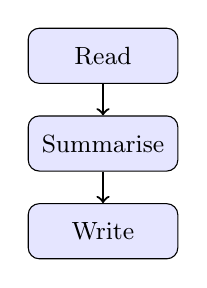
\begin{tikzpicture}[
                node distance=0.4cm,
                blk/.style={draw, rounded corners, fill=blue!10,
                            minimum width=1.9cm, minimum height=0.7cm,
                            align=center, font=\small}]
                \node[blk] (a) {Read};
                \node[blk, below=of a] (b) {Summarise};
                \node[blk, below=of b] (c) {Write};
                \draw[->, thick] (a) -- (b);
                \draw[->, thick] (b) -- (c);
            \end{tikzpicture}
        \end{column}
    \end{columns}
\end{frame}

% Revealing a table ROW BY ROW with \onslide. Because \onslide is a switch,
% remember to reset it with \onslide<1-> at the end of the tabular.
\begin{frame}{A table revealed row by row}
    \begin{table}
    \begin{tabular}{l | c | c | c | c}
    Competitor Name & Swim & Cycle & Run & Total \\
    \hline \hline
    John T   & 13:04 & 24:15 & 18:34 & 55:53 \\
    \onslide<2-3> Norman P & 8:00  & 22:45 & 23:02 & 53:47 \\
    \onslide<3->  Alex K   & 14:00 & 28:00 & n/a   & n/a   \\
    \onslide<4->  Sarah H  & 9:22  & 21:10 & 24:03 & 54:35
    \onslide<1->
    \end{tabular}
    \caption{Triathlon results}
    \end{table}
\end{frame}


% =============================================================================
\section{Blocks and theorems}
% =============================================================================

% Three coloured boxes. All take a REQUIRED title argument.
\begin{frame}{The three block environments}
    \begin{block}{Real Madrid}
        Greatest football club in the world.
    \end{block}

    \begin{alertblock}{Surprising}
        Barcelona conceded 8 goals in one leg!
    \end{alertblock}

    \begin{exampleblock}{UCL Titles}
        RMA has 15 titles!
    \end{exampleblock}
\end{frame}

% GOTCHA -- a trap in the 2021 tutorial:
%   exampleblock  is the coloured BOX; its argument is a required title.
%   example       is a THEOREM-LIKE environment; its argument is an optional
%                 name in brackets.
% They are different things. Use exampleblock when you want the green box.
\begin{frame}{Theorem-like environments are pre-defined}
    % No \newtheorem needed -- beamer already defines theorem, corollary,
    % proof, definition, lemma, fact and example.
    \begin{theorem}[Pythagoras]
        $a^2 + b^2 = c^2$
    \end{theorem} \pause
    \begin{corollary}
        $x + y = y + x$
    \end{corollary} \pause
    \begin{proof}
        $\omega + \phi = \epsilon$
    \end{proof}
\end{frame}

\begin{frame}{example vs exampleblock}
    \begin{example}[a theorem-like environment]
        Its argument is an optional NAME in brackets.
    \end{example}
    \begin{exampleblock}{a coloured box}
        Its argument is a required TITLE in braces.
    \end{exampleblock}
    \begin{definition}
        A definition.
    \end{definition}
\end{frame}


% =============================================================================
\section{Frame options}
% =============================================================================

% GOTCHA: a frame containing verbatim, lstlisting or minted MUST be declared
% [fragile], or compilation fails with a confusing error.
\begin{frame}[fragile]{Code needs [fragile]}
\begin{lstlisting}[language=Python, basicstyle=\ttfamily\small,
                   frame=single, showstringspaces=false]
def writhe(signs):
    return sum(signs)
\end{lstlisting}
    Without \texttt{[fragile]} this frame does not compile.
\end{frame}

% [shrink=n]          scale the frame down by up to n percent if it overflows
% [allowframebreaks]  let the frame spill over onto extra slides
% [plain]             no headline, no footline -- for a full-bleed slide
% [t] [c] [b]         vertical alignment of the frame body
\begin{frame}[shrink=10]{[shrink=10] rescues an overflowing frame}
    If the content is slightly too tall, \texttt{shrink} scales it down
    rather than letting it run off the bottom. \texttt{allowframebreaks}
    is the alternative: it spills the frame onto extra slides and appends
    a roman numeral to the title.
\end{frame}

\begin{frame}[plain]{[plain] hides the headline and footline}
    Useful for a full-bleed image or a section divider.
\end{frame}

% TikZ works inside a frame with no extra setup, and understands overlays --
% the simplest approach is one \only<n>{...} per stage.
\begin{frame}{TikZ in a frame, staged with \texttt{\textbackslash only}}
    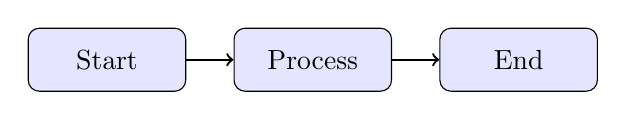
\begin{tikzpicture}[node distance=0.6cm,
        blk/.style={draw, rounded corners, fill=blue!10,
                    minimum width=2cm, minimum height=0.8cm, align=center}]
        \node[blk] (a) {Start};
        \node[blk, right=of a] (b) {Process};
        \only<2->{\node[blk, right=of b] (c) {End};}
        \draw[->, thick] (a) -- (b);
        \only<2->{\draw[->, thick] (b) -- (c);}
    \end{tikzpicture}
\end{frame}

\begin{frame}{Cheat sheet}
    \begin{itemize}
        \item \texttt{\textbackslash pause} -- everything after waits one click
        \item \texttt{<3-> <-3> <2-4> <1,3,5> <+->} -- overlay specifications
        \item \texttt{\textbackslash only} no space \textbar{}
              \texttt{\textbackslash uncover} / \texttt{\textbackslash visible} keep space
        \item \texttt{\textbackslash onslide<2->} -- a switch, reset it afterwards
        \item \texttt{block} / \texttt{alertblock} / \texttt{exampleblock}
        \item \texttt{[fragile]} for code, \texttt{[shrink=10]} for overflow,
              \texttt{[plain]} for full bleed
        \item \texttt{\textbackslash setbeamercovered\{transparent\}} -- dim, do not hide
        \item \texttt{\textbackslash setbeamertemplate\{navigation symbols\}\{\}} -- kill the arrows
    \end{itemize}
\end{frame}

\end{document}
